\documentclass{article}

% Packages
\usepackage[utf8]{inputenc}
\usepackage[english]{babel}
\usepackage[top=2cm, bottom=4.5cm, left=2.5cm, right=2.5cm]{geometry}
\usepackage{fancyhdr}
\usepackage{fullpage}
\usepackage{lastpage}
\usepackage{listings}
\usepackage{color}
\usepackage{tikz-er2}
\usepackage{float}

% Path to images
\graphicspath{ {./images/} }

% Debug Packages
\usepackage{blindtext}

% Code Design
\lstset{
   breaklines=true,
   basicstyle=\ttfamily,
   language=SQL,
   numbers=left,
   numberstyle=\tiny,
   commentstyle=\color{gray},
   keywordstyle=\color{blue},
   identifierstyle=\color{black}}

% ER Model Design
\usetikzlibrary{positioning}

% Title
\title{CanvasPath}
\author{Eric Roeum}

% Document
\begin{document}

  % Title
  \maketitle
  \pagenumbering{gobble}
  \newpage

  % Table of Contents
  \tableofcontents
  \addcontentsline{toc}{section}{References}
  \newpage

  % Table of Figures
  \listoffigures
  \newpage

  \pagenumbering{arabic}

  %%%%%%%%%%%%%%%%%%%%%%%%%%%%%%%%%%%%%%%%%%%%%%%%%%%%%%%%%%%%%%%%%%%%%%%%%%%%%%
  % Introduction:

  \section{Introduction}\label{sec:Introduction}
    At Lion State University, staff and students need a system in order to maintain information about classes, students, grades, roles, and other aspects of school.  Because of this, a database is required to hold all of this information in a usable format that student and teachers can access both easily and securely.  This system will be called CanvasPath.  The CanvasPath application will primarily be composed of four components:
    \begin{itemize}
        \item A login system
        \item Viewing courses
        \item Scheduling courses
        \item Deriving student infromation
    \end{itemize}
    As such, this system will be web browser based with a client-server implemented model.  The client system will only be used for input/output, while the server will handle all database operations.
    \newline\newline
    This system will be an updated version of the current applications: Canvas and LionPath.  By integrating both systems into one, users will have more ease of use and will be able to do operations in one system instead of having to switch between both.

  \medskip

  \subsection{Objective}\label{sec:Introduction:Objective}
    The purpose of the document is to propose an implmentation for the CanvasPath application along with potential features.  In addition to doing so, this document contains how the internal database should be organized along with potential designs.  As a result, this document is divided primarily into five components:
    \begin{itemize}
      \item Requirements analysis
      \item Web Application Design
      \item Conceptual database design
      \item Technological survey
      \item Logical database design
      \item Schema Refinements
    \end{itemize}

  \medskip

  \subsection{Stylization}\label{sec:Introduction:Stylization}
    Within this document, certain styles and notations will be used for readability.  More specifically, italicization is resevered for only variable names (i.e. \textit{Height}).  Any other forms of text can be used in any other context.  For entity-relationship (ER) diagrams, the textbook notation is used (See reference \cite{textbook}).

  \newpage

  %%%%%%%%%%%%%%%%%%%%%%%%%%%%%%%%%%%%%%%%%%%%%%%%%%%%%%%%%%%%%%%%%%%%%%%%%%%%%%
  % Requirements Analysis

  \section{Requirements Analysis}\label{sec:Requirements}
    This section goes over the requirements proposed by LionState University for the CanvasPath project.

  \subsection{Overview}\label{sec:Requrements:Overview}
    Because CanvasPath is intended to replace current course managements systems at LionState University, a lot of the requirements come from updating the features of the current system, Canvas and LionPath.  As such, CanvasPath requires a login system for the user to be identified, a system to control course scheduling/viewing, and accessing personal info primarily.  As a result, each system must be implemented in order to meet the requirements of the current application.  Of course, it is important to include new features as well.  However, current features need to be implemented before new features should be developed.

  \subsection{System Overview}\label{sec:Requirements:System}
    In terms of easibility, Canvas has the advantage over Lionpath, so the overall system should mimic the Canvas system more so.  As a result, the canvas design flow will be followed.  When the user first opens the application, for example, they are presented with a login screen such that they can identify who they are without allowing others to access the same information.  After logging in, the system should detect if the user is a student, faculty member, or administrator.
    \newline\newline
    Each user will be presented with three levels of usability:
    \begin{itemize}
      \item A student can view and sign-up for classes
      \item A faculty member can view, sign-up, and create classes/groups
      \item An administrator can do everything a student and faculty member can do, but also create new users.
    \end{itemize}
    Another aspect that canvas has is viewing individual course details.  Within each course, students and faculty members should be able to view grades, announcments, assignmennts, files, grades, associated people, and view syllabi.
    \newline\newline
    Within LionPath, features unique to LionPath should also be added to this Canvas-like system.  For example, scheduling course, viewing available courses, prerequisite courses, academic records, tuition, and research activities.  As a result, after logging into the system, a user should be given a menu to choose the correct action.

  \subsection{Users}\label{sec:Requirements:Users}
    There are two primary users: a student and a faculty member, with the special user called the administrator.  Each category is not necessarily disjoint from each other though.  For example,  a student may also be a faculty member.  Both the student and faculty member should have personal information stored as well as courses taken/taught, grades, etc.  The primary difference between the two is that a student should take a class whereas a faculty member should support a class.
    \newline\newline
    A student is any person who is currently taking or has taken a class.  Because of this, each student requires past courses, current courses, future courses, grades, assignments, and files to be stored in order to meet this requirement academically.  On more personal levels, it is also important to store more personal information.  For example, a student's primary address, personal email, school email ID, passwords, emergency contacts are essential to keep.  Further relations need to be stored as well.  For example, the instructors, courses, sections, departments, etc. that the student is related to should alos be stored.
    \newline\newline
    On the other hand, any person who is currently supporting or has supported a class is a factuly member.  This includes, teachers, professors, researchers, teaching assistants, learning assistants, and more.  Faculty members are very similar in what data is required on them: past courses, current courses, future courses, files, research, budget, etc.  More information is then required for human resourse (HR) purposes: pay-rate, years worked, department.
    \newline\newline
    The final administrator user is particularly useful for implementing new groups and users.  These users will have full control to the system and are able to both access and manipulate any data.

    \subsubsection{Student}\label{sec:Requirements:Users:Student}
      A student is any user who is enrolled at Lion State University.  It is important to maintain information about enrolled students so both students and faculty members can enroll into courses appropriately.  Information stored about students should include:
      \begin{itemize}
        \item Name: Student Name
        \item ID: Student ID
        \item Age: Student Age
        \item Gender: Male/Female/Other
        \item Email Address: Personal email address of student
        \item Home Address: Permananent/Mailing address of student
        \item Login Password: Password to log into system (Encoded into SHA256)
        \item Majors/Minors: Completed/Intended graudation path of student
      \end{itemize}

    \subsubsection{Faculty Member}\label{sec:Requirements:Users:Faculty}
      A faculty member is any user who supports any course at Lion State University.  Note that courses may not necessarily be purely academic and supporting a course does not necessarily mean teaching a class.  Still, it is importannt to maintain information about active faculty member so that they can properly support their respective course.  Information stored about faculty members include the following:
      \begin{itemize}
        \item Name: Faculty Name
        \item ID: Faculty ID (Note that this is synonomous for Student ID as they come from the same pool of values)
        \item Age: Faculty Age
        \item Gender: Male/Female/Other
        \item Email Address: Personal email address of faculty member
        \item Home Address: Permananent/Mailing address of faculty member
        \item Login Password: Password to log into system (Also encoded into SHA256)
        \item Department: Department that faculty corresponds
        \item Pay-grade: Level of pay faculty member gets paid
        \item Semesters Working: Amount of years worked by faculty member
        \item Office Address: Working office of faculty member
        \item Title: Title of faculty member
      \end{itemize}

  \subsection{Groups}\label{sec:Requirements:Groups}
    In order to avoid duplication of data, groups are made to rerpresent areas where a group of individuals of users share a certain aspsect.  These groups are primarily categorized by the following:
    \begin{enumerate}
      \item Courses: a class which a student may take and a faculty member may teach/support.  Courses can only be offered by one department (though duplicate courses can have different departments i.e. CS/DS 200).  Within each course, the course name, course ID, department, sections, primary teacher, support staff, and students all need to be stored.
      \item Deparments: The certain degree program that classes identify with.  For example computer science, psychology, and engineering are considered as departments.  Note that duplicate departments cannot exist.  Within the department group, information regarding faculty members are mentioned as well as majors, minors, names of programs, etc.  The departments group individual courses by specific major/minor programs.
      \item Section: a subset of a course.  Because courses can be very large, it is important to maintain smaller groups in order to provide multiple sections of the same class.  Further, sections allow different course material.  For example, a capstone section can now be implemented in order to have different assignments.
    \end{enumerate}

  \subsubsection{Courses}\label{sec:Requirements:Groups:Courses}
    A course represents, not only a class that a student can take, but also an activity that some students or facilty members may participate in.  For example, a research activity can be considered a course, though it may not necessarily be for credit or have the ability enroll students.  However, using the research activity example, a single course will be implemented to represent all research activities on campus while each individual research activity is distibuted bia sections within the course information.

  \subsubsection{Departments}\label{sec:Requirements:Groups:Departments}
    A department is a certain group which courses can associatite with, more specifically by majors.  For example, computer science, psychology, math, physics are all appropriate departments, though none of them have to necessarily be degree program offered by the university.  Further, administration may be able to control department budgets and activities of courses thorugh a single entity instead of controling each individaul activity.

  \subsubsection{Section}\label{sec:Requirements:Groups:Section}
    A section is a subset of a single course that a student can enroll.  Usually, sections of the same course vary in time, but not necessarily.  Further a section specifies the type of the course.  For example sections can represent the following:
    \begin{itemize}
      \item Regular: A class where students physically attend the course
      \item Online: A class where student access course information electronically
      \item Hybrid: A mixture of both regular and online classes
      \item Research: A research opportunity that students/faculty members can participate
      \item Internship: An opportunity that students can take off school during a semester term.
      \item Coop: An opportunity that students can take off school during multiple semester terms.
    \end{itemize}

    \newpage

  %%%%%%%%%%%%%%%%%%%%%%%%%%%%%%%%%%%%%%%%%%%%%%%%%%%%%%%%%%%%%%%%%%%%%%%%%%%%%%
  % Web Application Design

  \section{Web Application Design}\label{sec:Web}
    This section will cover the inteded design and implmentation for CanvasPath.  The web application will primarily be controlled via a server-client communication protocal, where all client-side operations will occur through a web browser.

  \subsection{Webpage Overview}\label{sec:Web:Overview}
    As stated previously all communcations will follow the server-client communication protocal.  The client-side of this application will be the highlight of this section.  Within this aspect, there are four primary windows:
    \begin{itemize}
      \item Login Screen
      \item Homepage
      \item Personal Information
      \item Current Schedule
      \item Class Scheduler
      \item Finances
    \end{itemize}
    The following diagram shows how each window should interfaces with one another.  The first screen any user is presented with is the login screen.  Afterwards, any window that the current window is pointing towards can be accessed.

    \begin{figure}[h]
    \begin{center}
    \scalebox{0.87}{
    \begin{tikzpicture}[node distance=1.5cm, every edge/.style={link}]

      \node[entity] (logn) {Login};
      \node[entity] (home) [below=of logn] {Homepage};
      \node[entity] (info) [left=of home] {Personal Info};
      \node[entity] (schd) [below left=of home] {Current Courses};
      \node[entity] (schl) [below right=of home] {Class Scheduler};
      \node[entity] (fins) [right=of home] {Finances};

      \draw[<->] (logn) edge node {} (home);
      \draw[<->] (info) edge node {} (home);
      \draw[<->] (schd) edge node {} (home);
      \draw[<->] (schl) edge node {} (home);
      \draw[<->] (fins) edge node {} (home);

      \draw[->] (info) edge node {} (logn);
      \draw[->] (schd) edge node {} (logn);
      \draw[->] (schl) edge node {} (logn);
      \draw[->] (fins) edge node {} (logn);

    \end{tikzpicture}
    }
    \caption{Flow Diagram of Webpage Screens}\label{fig:WebFlow}
    \end{center}
    \end{figure}

    \subsection{Login Screen}\label{sec:Web:Login}
      The login screen's only purpose is to allow users to identify themselves securily.  In order to avoid any confusion, this procedure is kept simple with two textboxes: the user id and password; and a button: submit request.  Though currently, the Canvas and LionPath applications have a "Forgot Password" button, this feature will not be added in order to reduce complications and stay in the scope of the assignment.

      \begin{figure}[H]
        \centering
        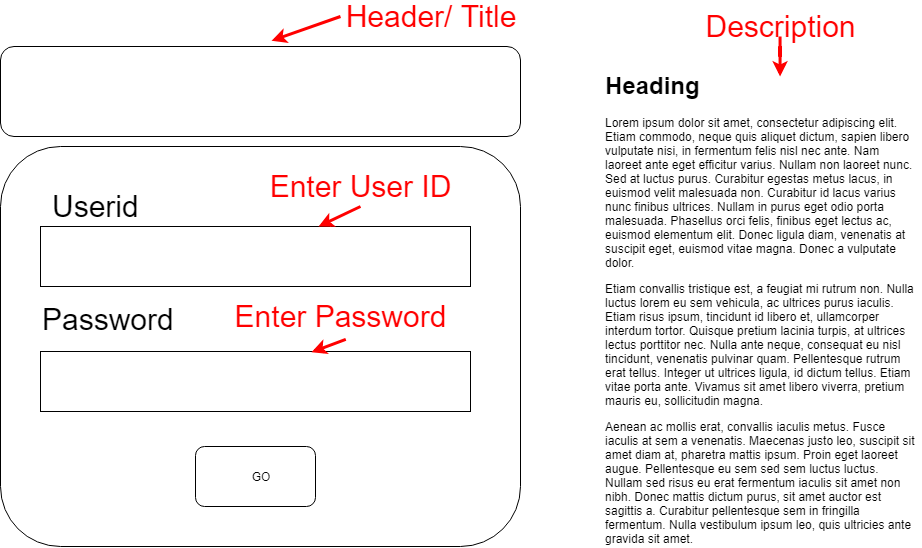
\includegraphics[width=4 in]{Design/LoginScreen}
        \caption{Login Webpage}
        \label{fig:login}
      \end{figure}

    \subsection{Homepage}\label{sec:Web:Home}
      The homepage is very similar to Canvas's Dashborad page.  This page will take the most recent activity for the user and display it on the screen such that it is very easy to view and use the most likely activity.  Further the homeage acts as a hub for the rest of the webpages; all webpages can be access from the home webpage.

      \begin{figure}[H]
        \centering
        \includegraphics[width=4 in]{Design/Homepage}
        \caption{Homepage}
        \label{fig:home}
      \end{figure}

    \subsection{Personal Infromation}\label{sec:Web:Personal}
      The personal information screen allows the user to both access and manipulate any personal data stored by the system.  For example, if the user wishes to change his/her password, address, phone number, and others, he/she can do so in the personal information webpage.  This page is also very simple: a table shows all the currently stored data.  After each row, a button is present that allows the user to change the respective field by enabling the textbox.  While changing information, two new buttons appear in order to either "confirm" or "cancel" the change.  On the top of the screen, there exists tabs in order to scroll through possible categories such as academics, finances, contact infromation, etc.  This webpage exists primarily as an archival page for older information.

      \begin{figure}[H]
        \centering
        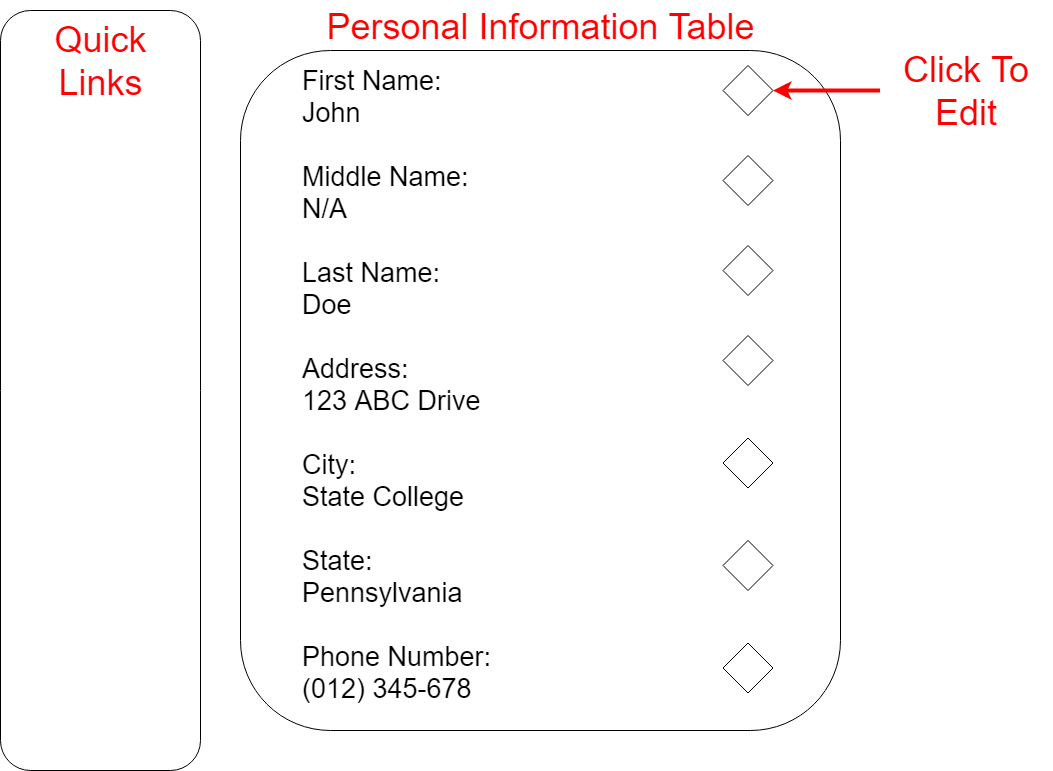
\includegraphics[width=5 in]{Design/PersonalInfo}
        \caption{Personal Information Webpage}
        \label{fig:personalinfo}
      \end{figure}

    \subsection{Current Schedule}\label{sec:Web:CSchedule}
      The current schedule provides students and faculty members access to current classes.  In this webpages, each student can view all of his/her courses, enter the specific course, and do anything relevant to that class.  This is most similar to Canvas's "Courses" tab.  Students and faculty members can access enrolled courses and see upcoming assignments, view any announcements, check grades, view files, etc.  Faculy members have special priveledes, however.  They can, for example, create announcements, upload files, and change grades.
      \newline\newline
      This page has a very simple design.  On the left-hand-side, there exists tabs to get to other screen.  In the center, a table displays all currently enrolled courses.  If a user selects a course in that table, the table disappears and that course's specific course page becomes active.

      \begin{figure}[H]
        \centering
        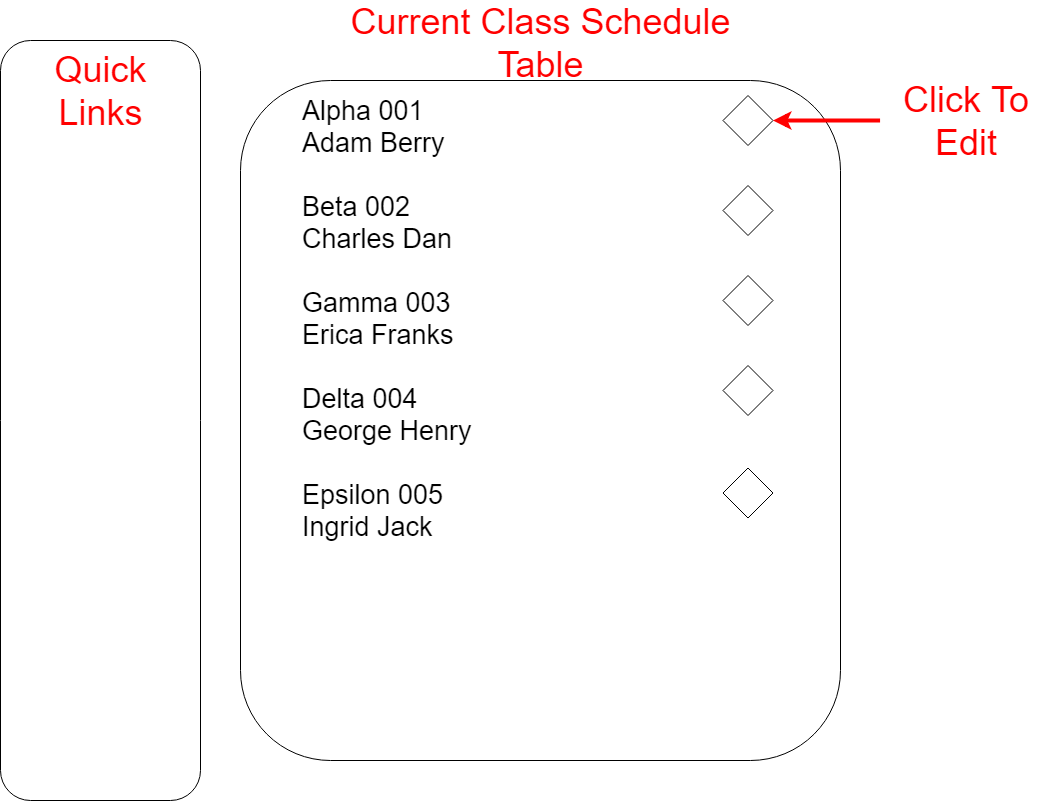
\includegraphics[width=4 in]{Design/ClassSchedule/Table}
        \caption{Table of currently enrolled courses}
        \label{fig:CScheduleTable}
      \end{figure}

      \begin{figure}[H]
        \centering
        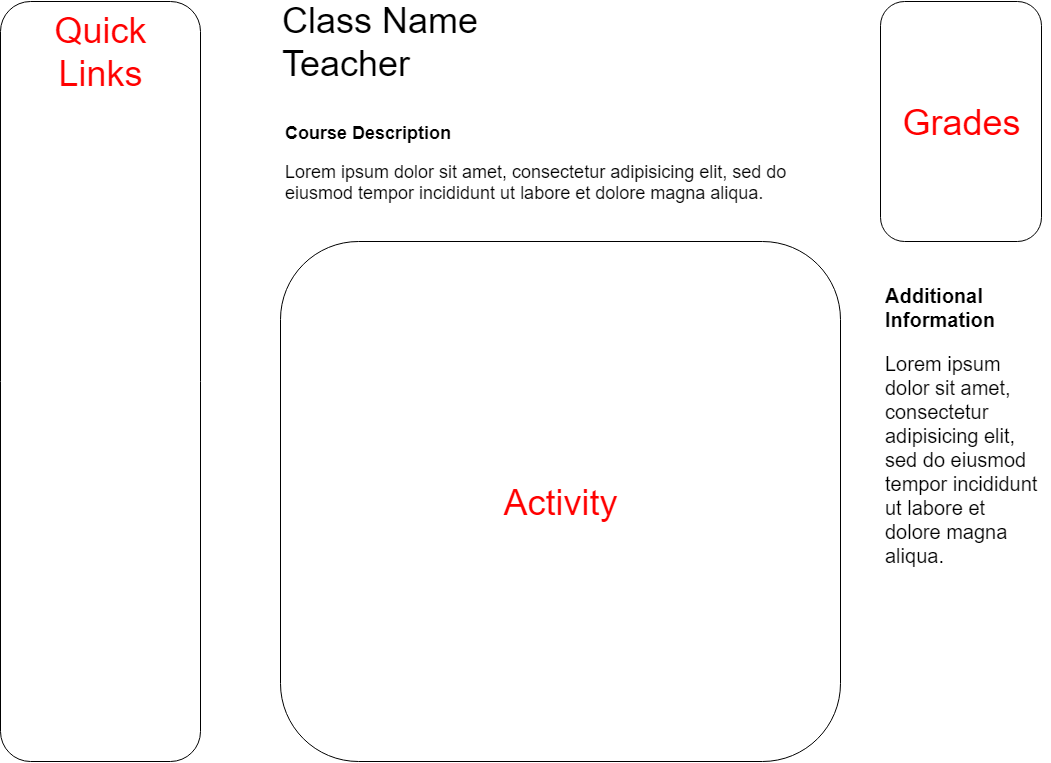
\includegraphics[width=4 in]{Design/ClassSchedule/CoursePage}
        \caption{Example of a course page}
        \label{fig:CSchedulePage}
      \end{figure}

    \subsection{Class Scheduler}\label{sec:Web:CScheduler}
      The class scheduler allows students to schedule for courses for future semesters as well as faculty members to create courses.  Any course that a student schedules must be approved by the instructor of the course.  Any course that a faculty member creates must be approved by an administrator.  This most closely follows LionPath's Scheduler Builder tool, combined with the "Search Classes" screen.  Following a similar design, the CanvasPath application will follow a folder system: classes are organized per department per semester.  The page is very similar to the current schedule page mentioned in section \ref{sec:Web:CSchedule}.

      \begin{figure}[H]
        \centering
        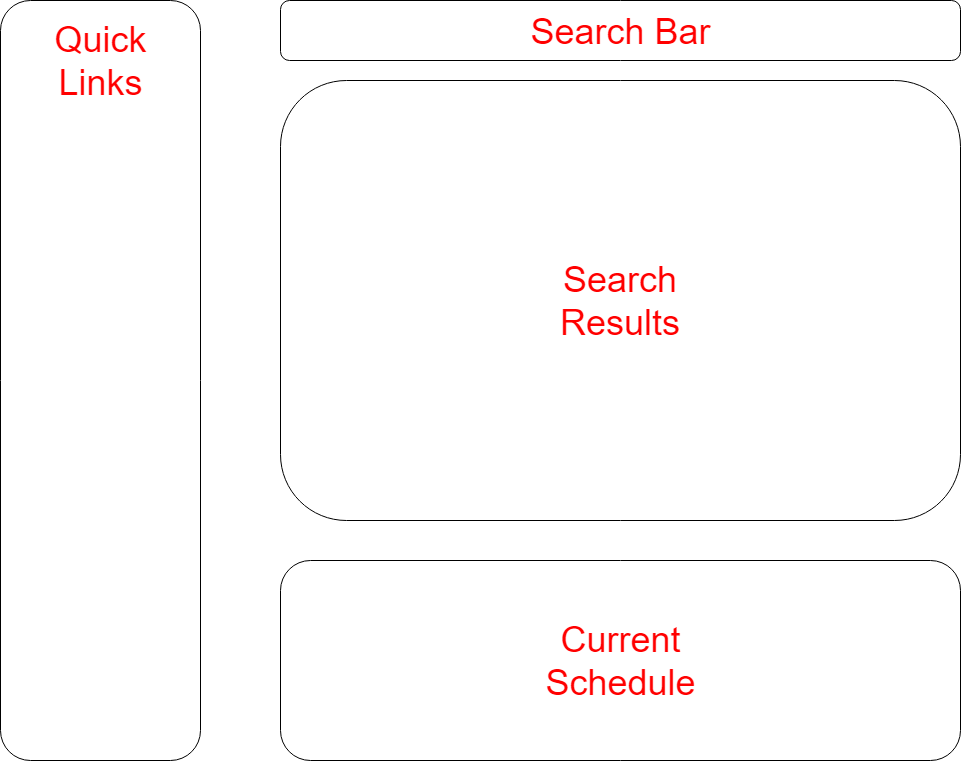
\includegraphics[width=4 in]{Design/CourseScheduler}
        \caption{Table of currently enrolled courses}
        \label{fig:CSchedule-Tasks}
      \end{figure}

      Within this class scheduler, a search bar is at the top of the page in order to search for the class desired.  Any results matching that string will be displayed in the search results window, where users can get more information on each specific course.  If the user is interested, he/she can add that to his/her current schedule, displayed at the bottom.  Any course added, is then requested to the instructor of the course for approval.  At the start of the semester, any student who was denied entry to the course or is still waiting is removed from this menu.  Note that any courses not added to the current schedule are not saved, so the user must research for the course.  A faculty member has the additional feature to add to the course lists.  Approval is required by an administrator however.

    \subsection{Finances}
      The finance web page displays anything related to money.  A student can view estimated tuitions, housing costs, and meal plans.  A faculty member has the ability to view his/her paygrade, any bills, past payments, any forms, and payment type.  Most of the fields are immutable by anyone except an administrator.  The webpage is very simple, with a single table to view the previously stated fields.
      \newline\newline
      For the purposes of this project, no information will be mutable and no payments are actually generated.  Doing so would add unnecessary complications and require actual finances.  Further, the finance page will not be completely accurate; due to the scope of this project, no pricing details will be implemented and the estimates will be completely fictional.

      \begin{figure}[H]
        \centering
        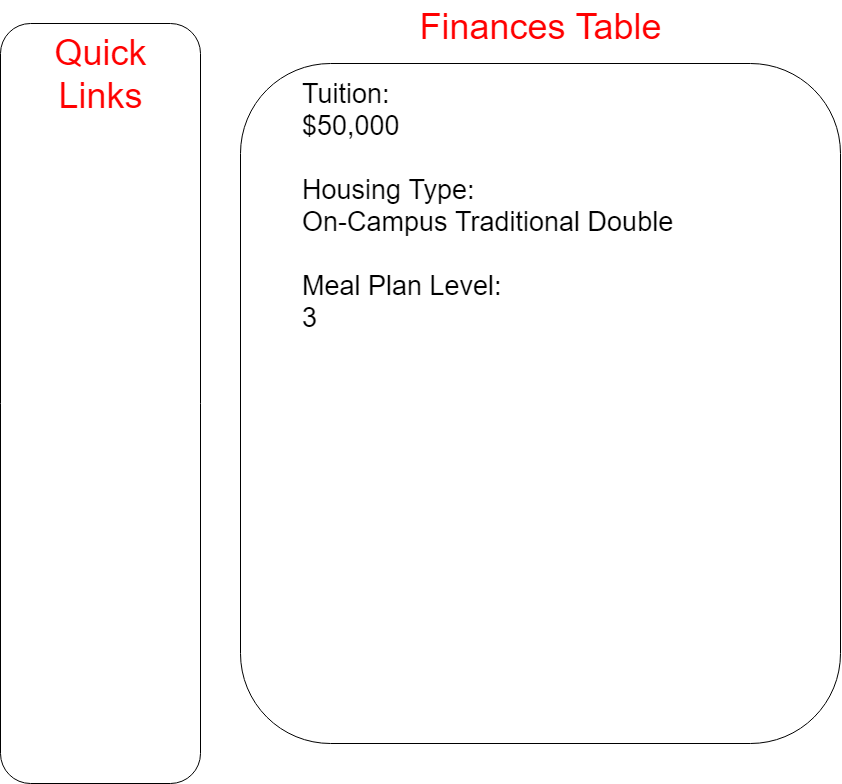
\includegraphics[width=4 in]{Design/Finances}
        \caption{Finances Webpage}
        \label{fig:Finances}
      \end{figure}

    \newpage

  %%%%%%%%%%%%%%%%%%%%%%%%%%%%%%%%%%%%%%%%%%%%%%%%%%%%%%%%%%%%%%%%%%%%%%%%%%%%%%
  % Appendix

  \section{Appendix}\label{sec:Appendix}

  \medskip

  %%%%%%%%%%%%%%%%%%%%%%%%%%%%%%%%%%%%%%%%%%%%%%%%%%%%%%%%%%%%%%%%%%%%%%%%%%%%%%
  % References

  \begin{thebibliography}{1}

    \bibitem{textbook}
    Ramakrishnan; Gehrke.
    \textit{Database Management Systems- Third Edition}.
    McGraw-Hill Higher Edication, 2003.

  \end{thebibliography}


\end{document}
